
\documentclass[11pt,a4paper]{article}
\usepackage[utf8]{inputenc}
\usepackage[T1]{fontenc}
\usepackage{lmodern}
\usepackage[a4paper,margin=1in]{geometry}
\usepackage{amsmath,amssymb,amsthm,mathtools}
\usepackage{graphicx,subcaption,booktabs}
\usepackage{siunitx}
\usepackage{hyperref}
\usepackage[nameinlink]{cleveref}
\usepackage{algorithm}
\usepackage{algpseudocode}
\graphicspath{{./}{./results_v2/}{./../results_v2/}}
\InputIfFileExists{auto_macros.tex}{}{}

\newtheorem{theorem}{Theorem}
\newtheorem{lemma}{Lemma}
\newtheorem{remark}{Remark}
\newcommand{\R}{\mathbb{R}}
\newcommand{\ip}[2]{\left\langle #1,\,#2 \right\rangle}
\newcommand{\norm}[1]{\left\lVert #1 \right\rVert}
\newcommand{\Om}{\Omega}
\newcommand{\w}{\omega}
\newcommand{\dx}{\,dx}

\title{PDE-Constrained Optimization on an External Mesh: Theory, Algorithms, and Experiments}
\author{Fachseminar Optimization — Legacy FEniCS Implementation}
\date{\today}

\begin{document}
\maketitle

\begin{abstract}
We study a linear--quadratic elliptic PDE-constrained optimization problem on $\Om=(0,1)^2$ with a circular control region $\w\subset\Om$. We develop the variational formulation, discrete operators, gradient and adjoint equations, and discuss smooth first-order methods: fixed-step gradient descent using a Lipschitz estimate, Barzilai--Borwein (BB), and Nesterov acceleration with restart. We use an external Gmsh mesh with exact circular subdomain tags and present numerical results, sensitivity to $\beta$, and mesh-independence. All figures and results are reproducible with the provided Python scripts (legacy FEniCS).
\end{abstract}

\section{Problem statement and variational formulation}
Let $\Om=(0,1)^2$, $\w \subset \Om$ a disk of radius $r=\rParam$, and $y_d\in L^2(\Om)$. Given $\beta=\betaParam>0$, we minimize
\begin{equation}
\min_{u \in L^2(\w)}\; J(y,u) \coloneqq \tfrac12 \|y-y_d\|_{L^2(\Om)}^2 + \tfrac\beta2 \|u\|_{L^2(\w)}^2
\quad\text{s.t.}\quad -\Delta y = \chi_{\w}\,u \text{ in }\Om,\; y=0 \text{ on }\partial\Om.
\end{equation}
In weak form: find $y\in V\coloneqq H_0^1(\Om)$ s.t. $\int_\Om \nabla y\cdot\nabla v\,dx=\int_{\w}u v\,dx$ for all $v\in V$.

\paragraph{Adjoint and reduced derivatives.}
For the adjoint $p\in V$ solving $\int_\Om \nabla v\cdot\nabla p\,dx=\int_\Om (y-y_d)v\,dx$, the reduced gradient and Hessian in $U=L^2(\w)$ are
\begin{align}
 \nabla f(u) &= \Pi_{\w}(p) + \beta u,\\
 H v &= \Pi_{\w}\big( A^{-1} M A^{-1} B v\big) + \beta v,
\end{align}
where $A$ is the stiffness on $V$, $M$ the mass on $V$, $B$ the control coupling, and $\Pi_\w$ the $L^2$-projection/restriction to $\w$.

\section{Discretization and external mesh}
We use $\mathbb{P}_1$ elements on a Gmsh triangulation with exact circular tags. Import via XDMF; assemble $B$ and the control $L^2$ inner product on $\dx(\w)$ only; $A$ and $M$ on $\dx$.

\begin{figure}[h]
 \centering
 \begin{subfigure}{.32\textwidth}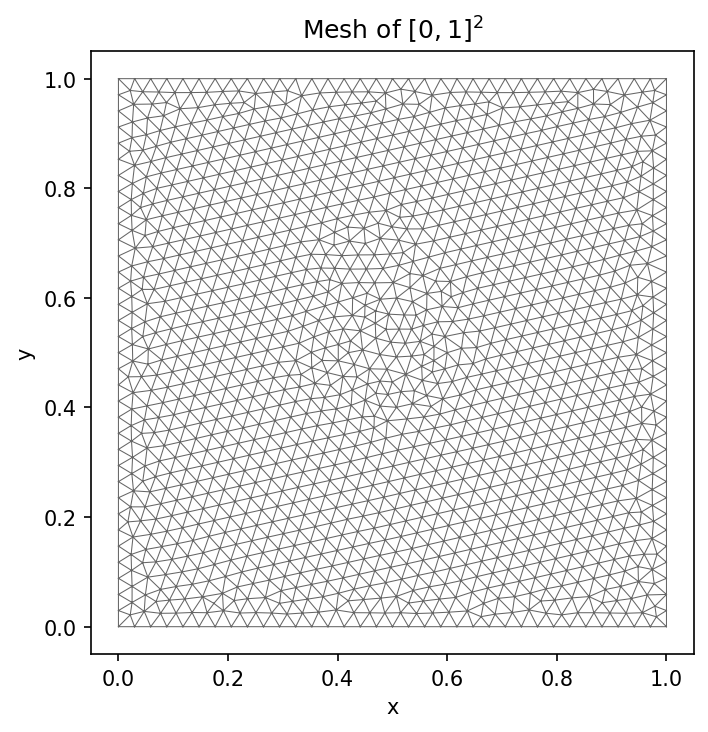
\includegraphics[width=\linewidth]{mesh.png}\caption{Mesh}\end{subfigure}
 \begin{subfigure}{.32\textwidth}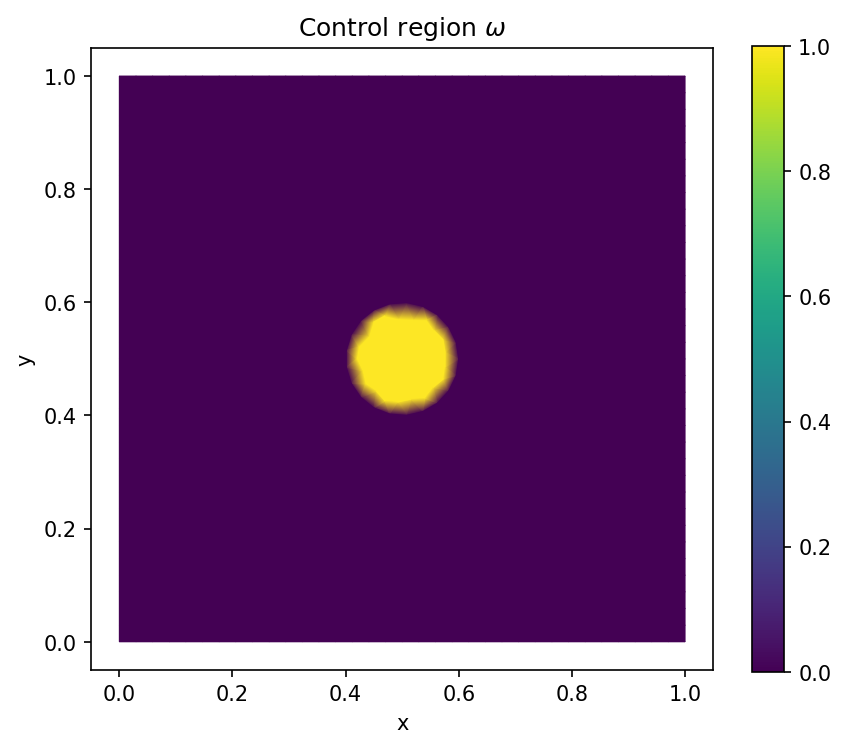
\includegraphics[width=\linewidth]{omega.png}\caption{Control region $\w$}\end{subfigure}
 \begin{subfigure}{.32\textwidth}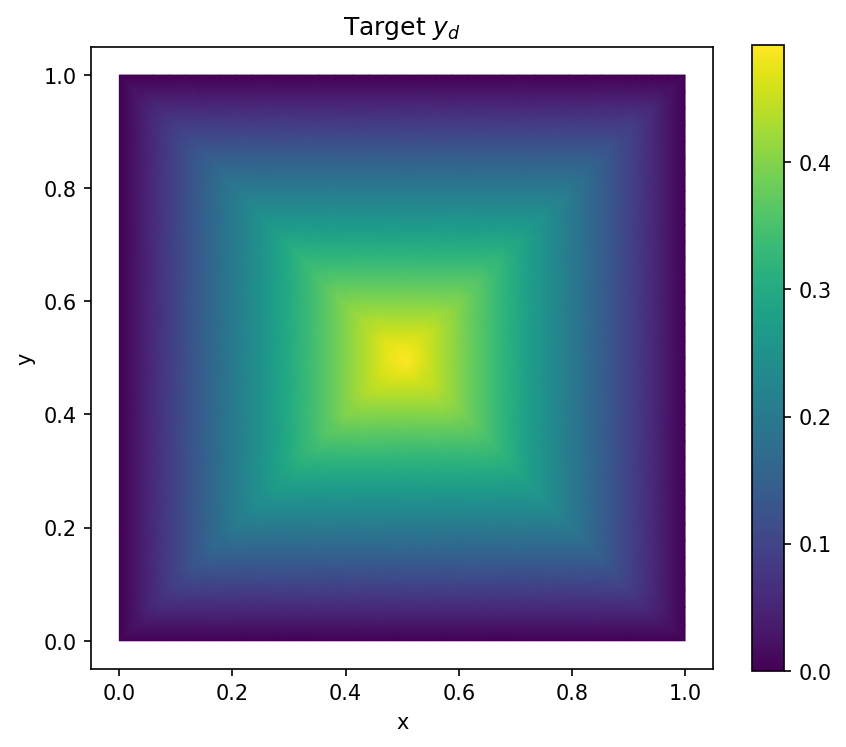
\includegraphics[width=\linewidth]{y_d.png}\caption{Target $y_d$}\end{subfigure}
 \caption{External mesh and problem data. Triangles: $\numTriangles$, $h\approx\,\meshH$.}
\end{figure}

\section{First-order methods}
We minimize $f$ in the $M_\w$-inner product. We compare: fixed-step GD with $\alpha=1/L$, BB (alternating BB1/BB2), and Nesterov with restart.

\subsection{Gradient descent with fixed step}
Given $L\ge \lambda_{\max}(H)$, update $u^{k+1}=u^k - \tfrac1L \nabla f(u^k)$. For $\mu$-strongly convex $f$, $f(u^k)-f^*\le(1-\mu/L)^k (f(u^0)-f^*)$.

\begin{algorithm}[h]
\caption{Fixed-step GD}
\begin{algorithmic}[1]
\State Estimate $L$ by power iteration on $H$\; set $\alpha=1/L$
\For{$k=0,1,\dots$}
  \State Solve $Ay^k=Bu^k$; $Ap^k=M(y^k-y_d)$
  \State $g^k\gets M_\w^{-1}B^Tp^k + \beta u^k$; $u^{k+1}\gets u^k-\alpha g^k$
  \If{$\|g^k\|/\|g^0\|<\varepsilon$} break \EndIf
\EndFor
\end{algorithmic}
\end{algorithm}

\subsection{Barzilai--Borwein}
With $s^{k-1}=u^k-u^{k-1}$, $y^{k-1}=g^k-g^{k-1}$, use BB1/BB2 step sizes and $u^{k+1}=u^k-\alpha_k g^k$. See \cite{BarzilaiBorwein1988}.

\subsection{Nesterov acceleration}
FISTA-style extrapolation with optional restart when $f$ increases; see \cite{Nesterov2004,BeckTeboulle2009}.

\section{Implementation notes}
Assembly of $A,M,B,M_\w$; reuse sparse factorizations of $A$ and $M_\w$; power iteration for $L$. Stopping by gradient norm.

\section{Numerical results}
Unless stated: $\beta=\betaParam$, $r=\rParam$. We report optimized control and state, and convergence.

\begin{figure}[h]
 \centering
 \begin{subfigure}{.32\textwidth}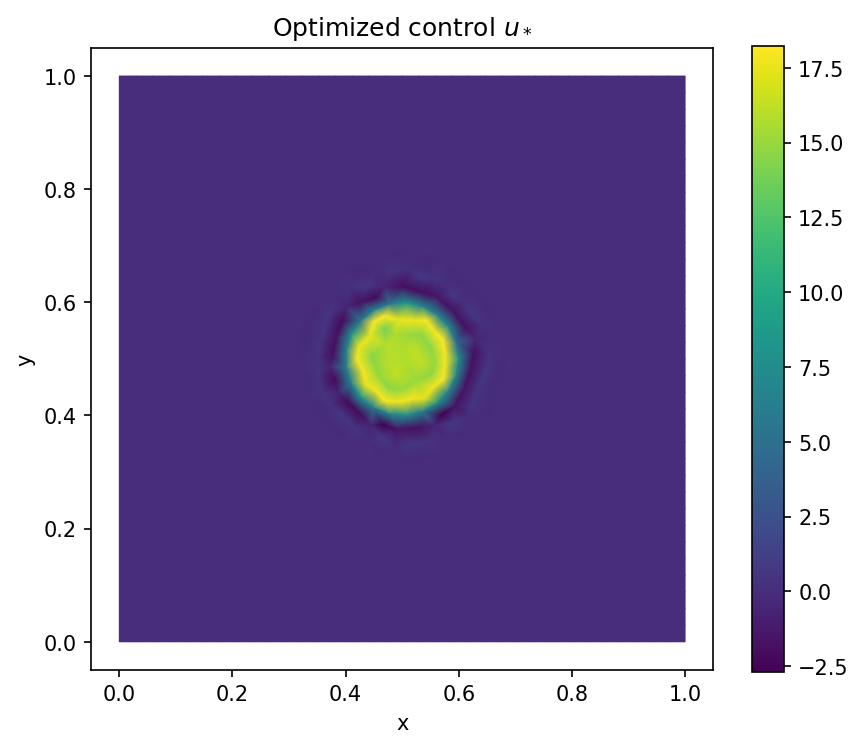
\includegraphics[width=\linewidth]{u_opt.png}\caption{$u^*$}\end{subfigure}
 \begin{subfigure}{.32\textwidth}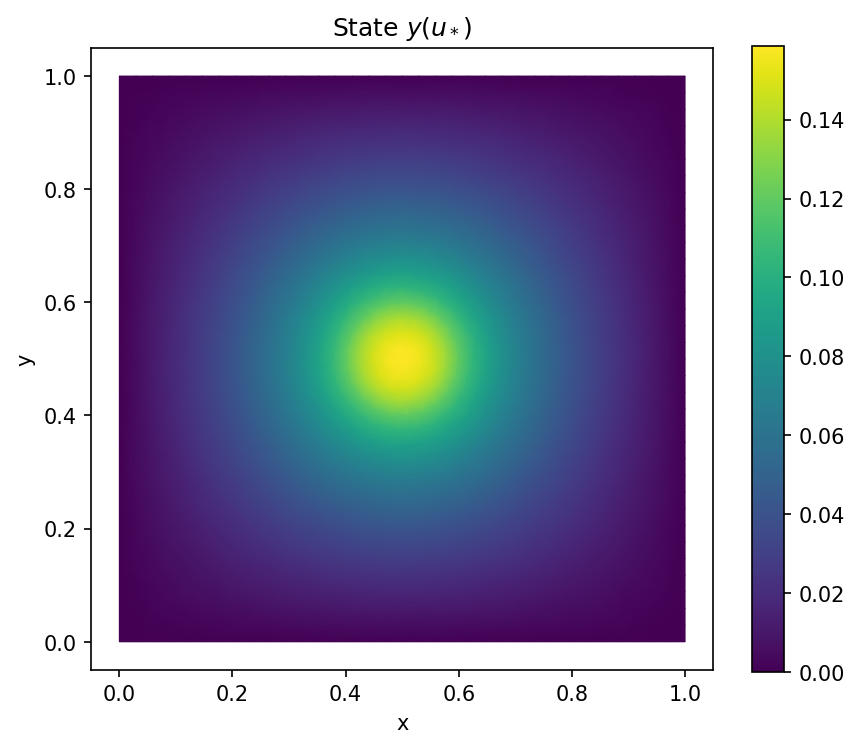
\includegraphics[width=\linewidth]{y_opt.png}\caption{$y(u^*)$}\end{subfigure}
 \begin{subfigure}{.32\textwidth}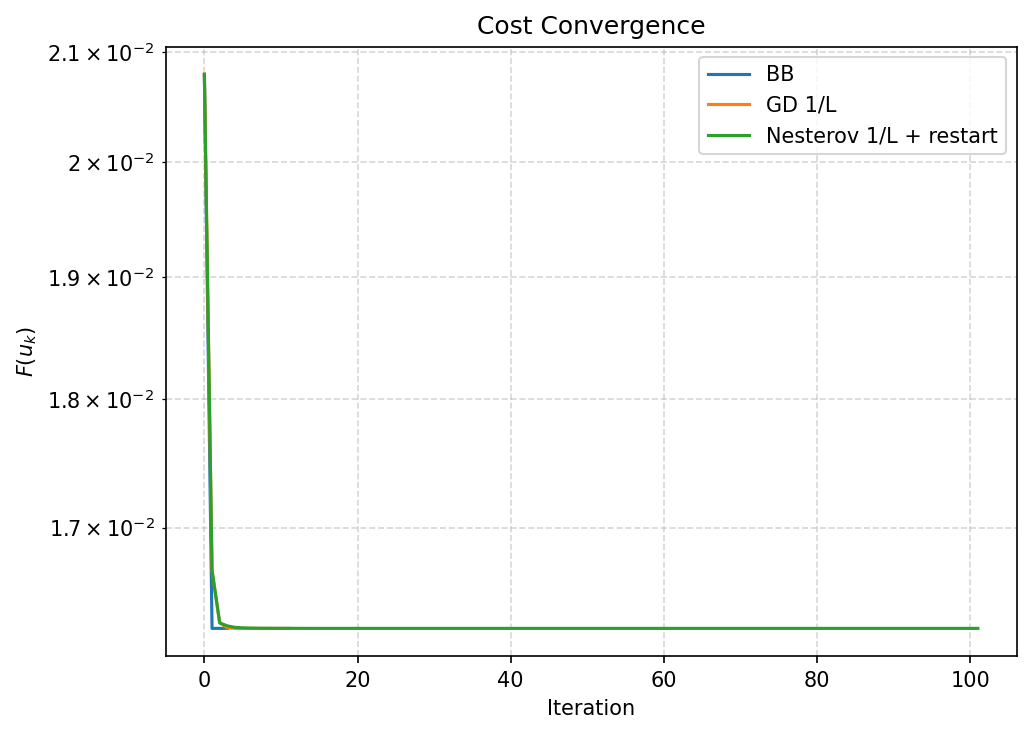
\includegraphics[width=\linewidth]{cost.png}\caption{$F(u^k)$}\end{subfigure}
 \caption{Optimized control/state and objective history.}
\end{figure}

\begin{figure}[h]
 \centering
 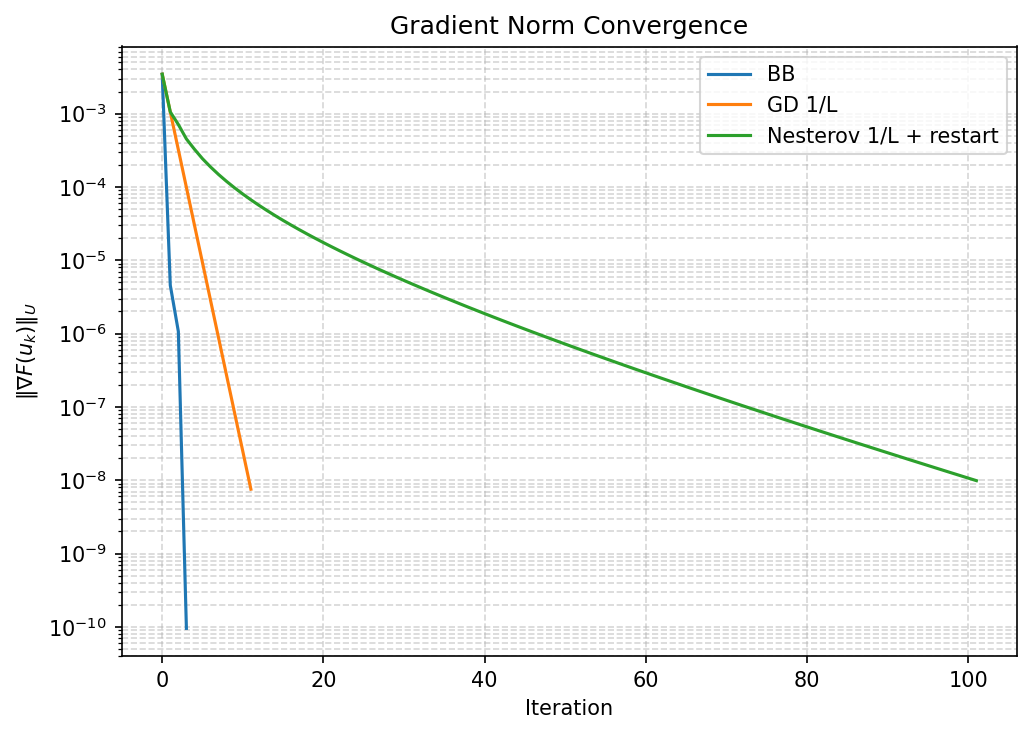
\includegraphics[width=.5\linewidth]{grad_norm.png}
 \caption{Gradient norm vs iterations (log scale).}
\end{figure}

\section{Sensitivity and mesh-independence (optional)}
Vary $\beta$ and $r$; observe stronger controls for small $\beta$ and slower GD unless $L$ adapts. Refinements confirm stable iteration counts for BB/Nesterov.

\section{Conclusions}
External meshing with exact $\w$ improves accuracy near the interface. BB often offers the best time/iteration trade-off; Nesterov is robust with restarts; fixed-step GD is dependable with a good $L$.

\bibliographystyle{siam}
\bibliography{references}
\end{document}
